\section{Exercise 3: StyleGan}

Look at this: \url{https://thispersondoesnotexist.com/} ! Would you
believe this picture is not real??? Well it is not! Feel free to refresh
the page to look at more examples. This picture has been generated by
\href{https://arxiv.org/pdf/1812.04948.pdf}{StyleGan}, a groundbreaking
architecture in the world of GANs! \newline

The StyleGan uses a lot of tricks that we have seen in the course (eg,
progressive growing) but also relies on a novel approach to controlled
generation. The figure below describes the architecture of the network: \newline

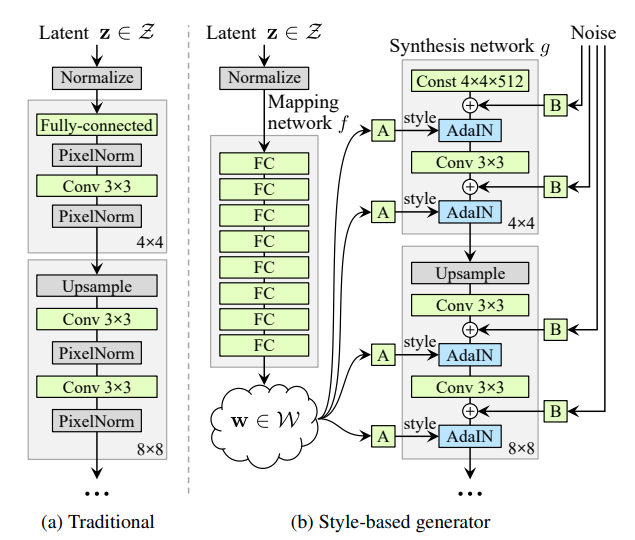
\includegraphics[width=1\linewidth]{img//genAdvNet//modernGAN/stylegan.png}

Wow! We have a completely new network in our GAN. This network is called
the \textbf{noise mapping} network. The architecture of this network is
fairly simple, it only consists of 8 fully connected layers. The authors
argue that mapping the latent vector \(z\) to a new latent vector \(w\)
facilitates \textbf{disentanglement}. \newline

We talked about disentanglement in the course: when modifying the latent
vector \(z\) to control the aspect of the generated image, we often face
entangled features. For example, longer hair can be correlated with a
more feminine face. Using the mapping vector in StyleGan facilities the
decorrelation of such features. \newline

What happens next? The generated \(w\) latent vector is injected into a
``classic'' generator network. However, this network has two components
you are not yet familiar with, as seen in the figure above. Indeed,
after each convolution layer, we see that the authors are adding
\textbf{noise}. Moreover, the convolution output with added noise is
then fed into a \textbf{adaptive instance normalization layer or AdaIN}.  \newline

In this notebook, you will implement a \textbf{noise injection layer}
and the \textbf{AdaIn layer}.

\subsection{Noise injection}
The noise injection helps with something that the authors call
\textbf{stochastic variation}. They argue that many aspects of a human
face are stochastic, such as hair curls or freckles. By adding random
noise at different levels in the generator, they can create more
variability without changing the overall image. For example in the image
below, we can see how different noise vectors impacts the placement of
the hair.

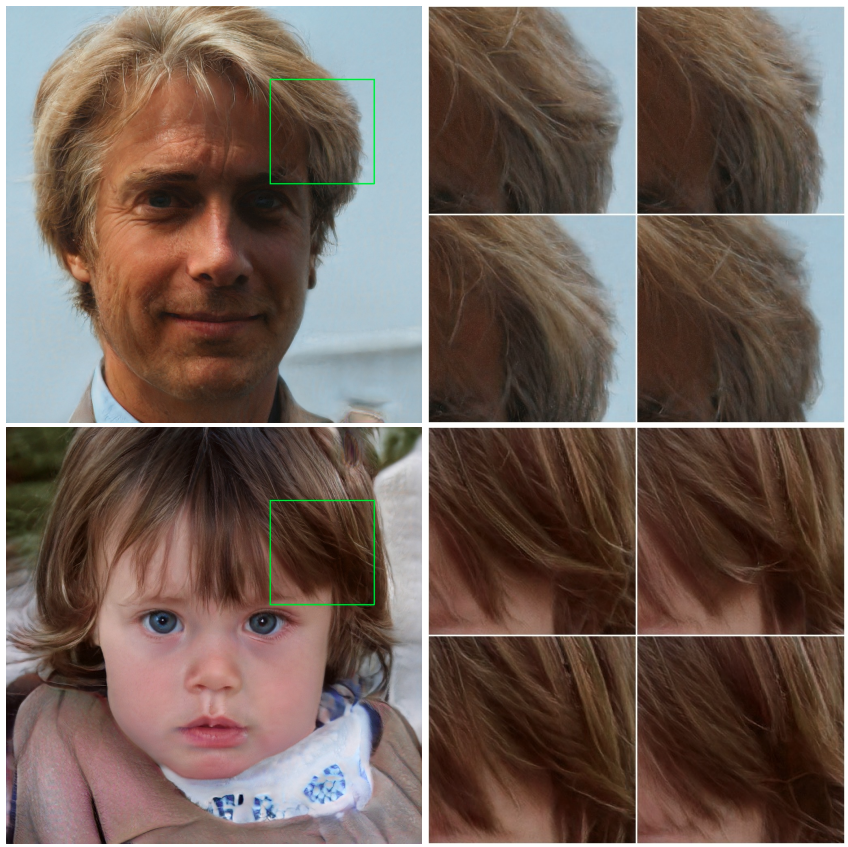
\includegraphics[width=0.5\linewidth]{img//genAdvNet//modernGAN/stochastic_variation.png}

After each convolution layer in the generator, the authors added a noise
injection layer. A random gaussian noise is added to the output and
scaled by a learned factor. Let's look at an example together: 
\begin{itemize}
    \item let's say that the output shape of the convolution layer is \lstinline{(1, 256, 32, 32)} where 256 is the number of channels and 32x32 the spatial dimensions.
    \item we create a random noise matrix of dimensions \lstinline{(1, 1, 32, 32)}
    \item we multiply the above random by a learned scaling factor vector of dimensions \lstinline{(1, 256, 1, 1)}. This learned scaling factor is initialized with zeros.
\end{itemize}

For the first exercise of this notebook, you will implement the
\lstinline{ApplyNoise} layer.

Click for tips

\begin{itemize}
\item You can read about custom pytorch modules implementation \href{https://pytorch.org/tutorials/beginner/examples_nn/two_layer_net_module.html}{here}.
\end{itemize}

\begin{lstlisting}[language=Python]
import torch
import torch.nn as nn

import tests
\end{lstlisting}

\begin{lstlisting}[language=Python]
class ApplyNoise(nn.Module):
    """
    Noise injection layer with learnable parameters.
    
    args:
    - channels: number of channels of the input
    """
    def __init__(self, channels: int):
        super(ApplyNoise, self).__init__()
        self.channels = channels
        self.weights = nn.Parameter(torch.zeros(1, channels, 1, 1))
    
    def forward(self, x: torch.Tensor) -> torch.Tensor:
        noise = torch.randn(1, 1, x.shape[2], x.shape[3])
        x = x + self.weights * noise
        return x
\end{lstlisting}

\begin{lstlisting}[language=Python]
apply_noise = ApplyNoise(512)
\end{lstlisting}

\begin{lstlisting}[language=Python]
tests.check_apply_noise(apply_noise)
\end{lstlisting}

\begin{lstlisting}
Congrats, you successfully implemented a noise injection layer!
\end{lstlisting}

\subsection{Adaptive instance normalization}
The Adaptive instance normalization (AdaIN) is a variation of the
\textbf{Instance Normalization layer}. In the course, we have discussed
about the importance of Batch Normalizations layers. However, we also
have seen that in some cases (eg, when using gradient penalties), Batch
Normalization is not the preferred type of normalization layer. \newline

This figure from the \href{https://arxiv.org/pdf/1803.08494.pdf}{Group
Normalization} paper helps to understand the differences between the
normalization layers. In the figure below, \(H\) and \(W\) are the
spatial dimensions, \(C\) the channel dimension and \(N\) the batch
dimension.

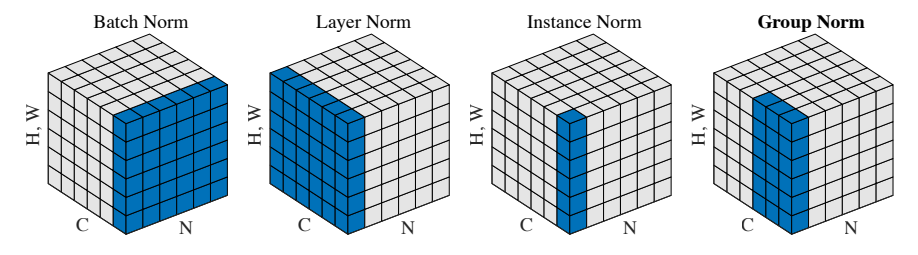
\includegraphics[width=1\linewidth]{img//genAdvNet//modernGAN/normalization_layers.png}

In\href{https://pytorch.org/docs/stable/generated/torch.nn.BatchNorm2d.html}{\textbf{Batch Normalization}}, we normalize pixels of the same channel, accross the batch and spatial dimensions. \newline

In \href{https://pytorch.org/docs/stable/generated/torch.nn.LayerNorm.html}{\textbf{Layer Normalization}}, we normalize pixels of the same batch index, accross the channel and spatial dimensions. \newline

In \href{https://pytorch.org/docs/stable/generated/torch.nn.InstanceNorm2d.html}{\textbf{Instance Normalization}}, we normalize pixels of the same batch index and channel, accross the spatial dimensions only. \newline

In \href{https://pytorch.org/docs/stable/generated/torch.nn.GroupNorm.html}{\textbf{Group Normalization}}, we group pixels of the batch index together. \newline

The AdaIN layer is an extension of the Instance Normalization layer. It
takes as input both the output of the previous convolution layer and the
latent vector \(w\). Then it performs the following: 
\begin{itemize}
    \item map the latent vector \(w\) to styles vector \((y_{s}, y_{b})\) through learned affine transformations (fully connected layers).
    \item calculate the output of the layer using the following equation: \(y_{s} * In(x) + y_{b}\) where \(In(x)\) is the input \(x\) fed through an instance normalization layer.
\end{itemize}

For the second exercise in this notebook, you will implement the AdaIN
layer.

\textbf{Tip:}

\begin{itemize}
\item You can use the torch Instance Normalization module for an easier implementation.
\end{itemize}

\begin{lstlisting}[language=Python]
class AdaIN(nn.Module):
    """
    Adaptive Instance Normalization layer
    
    args:
    - channels: number of channels of the input
    - w_dim: dimension of the latent vector w
    
    inputs:
    - x: float32 tensor of dim [N, C, H, W]
    - w: float32 tensor of dim [N, W_DIM]
    """
    def __init__(self, channels: int, w_dim: int):
        super(AdaIN, self).__init__()
        self.channels = channels
        self.w_dim = w_dim
        self.instance_norm  = nn.InstanceNorm2d(channels)
        self.linear_s = nn.Linear(w_dim, channels)
        self.linear_b = nn.Linear(w_dim, channels)
        
    def forward(self, x: torch.Tensor, w: torch.Tensor) -> torch.Tensor:
        x = self.instance_norm(x)       
        ys = self.linear_s(w)[..., None, None]
        yb = self.linear_b(w)[..., None, None]
        return x * ys + yb
\end{lstlisting}

\begin{lstlisting}[language=Python]
adain = AdaIN(512, 128)
\end{lstlisting}

\begin{lstlisting}[language=Python]
tests.check_adain(adain)
\end{lstlisting}

\begin{lstlisting}
Congrats, you successfully implemented the AdaIN layer!
\end{lstlisting}
